\documentclass[preprint,12pt]{elsarticle}

\usepackage{lmodern}
\usepackage{amsmath}
\usepackage{amssymb}
\usepackage{graphicx}
\usepackage{booktabs}
\usepackage{tabularx}
\usepackage{array}
\usepackage{makecell}
\usepackage{multirow}
\usepackage{xcolor}
\usepackage{url}
\setlength{\emergencystretch}{3em}
\Urlmuskip=0mu plus 2mu\relax

\graphicspath{{figures/}}

% --------------------------------------------------------------
% DRAFT-ONLY ANNOTATIONS. Flip to \showtasksfalse for submission.
% --------------------------------------------------------------
\newif\ifshowtasks
\showtasksfalse

\newcommand{\TODO}[1]{\ifshowtasks\textcolor{red}{\textbf{[TODO: #1]}}\fi}

\journal{Artificial Intelligence in Medicine}

\begin{document}

\begin{frontmatter}

\title{Knowledge-Based Temporal Abstraction for Predicting Complications in Hospitalized Adults with Diabetes or Hyperglycemia}

\author[aff1]{Shahar Oded\corref{cor1}}
\ead{shahar.oded@post.bgu.ac.il}
\cortext[cor1]{Corresponding author.}
\author[aff1]{Yuval Shahar}
\author[aff1]{Erez Shalom}
\author[aff2,aff3]{Amir Bashkin}
\author[aff4,aff5]{Leonard Saiegh}
\author[aff6]{Dror Cantrell}
\author[aff7]{Irit Wirsansky}
\author[aff2,aff8]{Muhamad Badarne}
\author[aff9]{Irena Barash}
\author[aff10,aff11]{Avivit Cahn}
\author[aff4,aff7]{Irit Hochberg}

\address[aff1]{Medical Informatics Research Center,
Ben-Gurion University of the Negev, Beer Sheva, Israel}
\address[aff2]{Azrieli Faculty of Medicine,
Bar-Ilan University, Safed, Israel}
\address[aff3]{Endocrinology and Diabetes Unit,
Galilee Medical Center, Nahariya, Israel}
\address[aff4]{Bruce Rappaport Faculty of Medicine,
Technion---Israel Institute of Technology, Haifa, Israel}
\address[aff5]{Endocrinology Institute,
Bnai Zion Medical Center, Haifa, Israel}
\address[aff6]{Internal Medicine Department C,
Shamir Medical Center, Beer Yaakov, Israel}
\address[aff7]{Endocrinology Unit,
Hillel Yaffe Medical Center, Hadera, Israel}
\address[aff8]{Endocrinology and Diabetes Service,
Tzafon Medical Center, Ramat Poriya, Israel}
\address[aff9]{Internal Medicine Department C,
Barzilai Medical Center, Ashkelon, Israel}
\address[aff10]{Internal Medicine Department A,
Hadassah Ein Kerem, Jerusalem, Israel}
\address[aff11]{Faculty of Medicine,
Hadassah Hebrew University Hospital, Jerusalem, Israel}

\begin{abstract}
\textbf{Objective.} INTERVenE temporal encoder previously predicted complications from clinical intervals in intensive care records. We examined whether the approach extends to general inpatient care and whether measures of adherence to inpatient diabetes-care guidelines add predictive information beyond the clinical history.

\textbf{Methods.} We used the first four days of admission at six Israeli general hospitals included in the Kineret project to predict eight outcomes through day 14, their recorded timing, and total length of stay. The mortality label included linked deaths up to 30 days after discharge, assigned to visit end. We compared logistic regression, supervised STraTS, and INTERVenE-Enc with either clinical intervals or statistically defined intervals (SAX). For each model family, we also tested whether adding scores and occurrence indicators for assessments of inpatient diabetes-care guidelines improved prediction. The test set comprised 4,508 admissions from 3,193 people. We estimated paired differences by resampling people.

\textbf{Results.} The clinical interval encoder achieved a support-weighted area under the precision--recall curve of 0.527, with paired gains of 0.053 over the raw-observation STraTS model (95\% CI 0.036--0.070) and 0.075 over logistic regression. Within the shared encoder architecture, clinical intervals also outperformed statistically defined intervals (SAX; 0.467; paired difference 0.060, 95\% CI 0.046--0.076). The advantage persisted at daily cutoffs from two to six days, and the encoder retained discrimination at each hospital held out from training. Guideline assessment modestly improved prediction of hyperglycemia, while the overall difference across outcomes was uncertain (0.007, 95\% CI $-0.003$ to 0.018).

\textbf{Conclusion.} Clinical intervals improved discrimination over a model of individual observations in both intensive care and general inpatient records, with models fitted in each health system. In the Kineret dataset, a knowledge base developed for inpatient diabetes care made it possible to trace contributions to predicted risk back to clinical trends and patterns of care. The predictive value of guideline assessment varied by outcome.
\end{abstract}

\begin{keyword}
knowledge based temporal abstractions \sep medium-term prediction \sep Transformers
\sep medical guideline adherence \sep electronic health records \sep inpatient diabetes
\end{keyword}

\end{frontmatter}

\IfFileExists{tasks.tex}{% Working notes are maintained in RESULTS_AUDIT.md and REVISION_NOTES.md.
\ifshowtasks
\noindent\fbox{\parbox{.95\linewidth}{Working draft. Confirm run provenance and clinical interpretation before submission. See RESULTS\_AUDIT.md.}}
\fi
}{}

\section{Introduction}
\label{sec:introduction}
Inpatient diabetes care involves changing glucose levels, treatment decisions, and measurements taken at intervals that vary across patients and clinical settings. A glucose value of 180 mg/dL, for example, may reflect persistent hyperglycemia or a rapid fall from a much higher level after insulin. Interpreting that value in context matters when estimating a patient's risk of subsequent complications.

Measurements can be interpreted in different ways. Knowledge-based temporal abstraction uses clinical rules to identify states, trends, and events in a patient's history \citep{shahar1997framework}. The same glucose readings, for example, can indicate both a high glucose state and a falling glucose trend. Statistical methods can also group measurements into intervals, using patterns in the data rather than clinical definitions. In the MIMIC-IV intensive care study, INTERVenE-Enc learned from both kinds of intervals and distinguished patients who developed complications more accurately than models of individual observations, including STraTS \citep{oded2026intervene,johnson2023mimiciv}.

Across six Israeli general hospitals in the Kineret network, a clinical study used a knowledge base developed for inpatient diabetes care to describe glucose trajectories and assess adherence to national treatmentrecommendations \citep{oded2027kineret-jbi,hochberg2023inpatient}. Greater adherence to the recommendation to give insulin after hyperglycemia was associated with less severe hyperglycemia, with only a slight increase in the risk of hypoglycemia. The same records allow us to ask a different question. Given what is already known about a patient's glucose levels and treatment, does an explicit assessment of adherence help predict a subsequent complication?

We used the first four days of each eligible Kineret admission to predict complications through day 14, their time of onset, and total length of stay. We examined INTERVenE-Enc in general inpatient care in a second health system, comparing its performance with models of individual measurements and testing what clinical intervals added over statistical intervals in the same encoder. We also assessed whether measures of adherence to inpatient diabetes-care guidelines added predictive information and examined how the encoder's named clinical patterns contributed to risk predictions.

\section{Background and related work}
\label{sec:background}
\subsection{Learning from irregular clinical observations}
A hospital record gives the time of a measurement more readily than the duration of the state it captures. GRU-D uses both missingness and the time elapsed since the last measurement \citep{che2018recurrent}. STraTS encodes the variable, value, and time of each observation and learns how observations relate to one another \citep{tipirneni2022strats}. Both can therefore use measurements taken at irregular intervals.

Knowledge-based temporal abstraction (KBTA) defines some of these relationships before model fitting \citep{shahar1997framework}. The Temporal Mediator applies the rules in a clinical knowledge base to time-stamped source concepts such as glucose measurements \citep{mediator-github}. It derives states, trends, events, and contexts, which may hold at a point in time or over an interval. The same glucose readings can contribute to two overlapping intervals, one indicating that glucose is high and the other that it is falling. Earlier methods identified recurring relationships between clinical intervals and used their frequencies and durations to predict outcomes \citep{moskovitch2015karmalego,sheetrit2019tpf}. INTERVenE represents the beginning and end of each interval separately, allowing the encoder to learn from duration and overlap while retaining the clinical identity of each interval \citep{oded2026intervene}.

\subsection{Representing guideline adherence over time}
The Kineret clinical study used the Temporal Mediator to assess fourteen components of inpatient diabetes care \citep{oded2027kineret-jbi,hochberg2023inpatient}. The Mediator then evaluates quality-assessment temporal patterns (QATPs) over the resulting clinical history. Each quality-assessment (QA) pattern specifies when a recommendation applies and what action is expected. For insulin after hyperglycemia, the assessment asks whether insulin was given during the period specified by the rule. For routine monitoring, the score depends on how often glucose was checked within a specified interval. These rules allow partial credit and can capture repeated assessments during a stay.

Two patients may have the same mean compliance score even if a missed or delayed action occurs at different points in their glucose trajectories. Kineret records both the scores and the intervals to which they refer. A model can therefore relate a particular assessment to the patient's course as well as use a summary of adherence up to the time of prediction.

\section{Methods}
\label{sec:methods}

\subsection{Study population and prediction time}
We used electronic health records from six Israeli general hospitals in the Kineret network for this retrospective study. The hospitals share a data warehouse based on the Observational Medical Outcomes Partnership common data model. Before abstraction, local measurement, medication, and observation codes were mapped to a shared clinical vocabulary and measurement units were harmonized \citep{oded2027kineret-jbi}.

The source cohort comprised adults admitted for 48 hours to 14 days with at least one overnight measurement (18:00--07:00). An admission qualified if the patient had a documented diabetes diagnosis or met either glucose criterion in the first 48 hours. The glucose criteria were two readings of at least 180 mg/dL taken 2--24 hours apart, or one reading of at least 250 mg/dL. The source study excluded admissions to pediatric and obstetric departments, deaths within 48 hours, and admissions with a duplicated visit identifier assigned to more than one person \citep{oded2027kineret-jbi}.

We chose 96 hours as the primary prediction time to allow repeated measurements and responses to treatment to enter the history. Both the raw and abstracted records had to extend beyond that point. The calendar dates came from the approved multicenter protocol for evaluating the national inpatient diabetes recommendations, issued in September 2023. That study drew on a period before implementation (August 2022--July 2023) and a later period allowing time for adoption (August 2024--December 2025) \citep{hochberg2023inpatient,oded2027kineret-jbi}. The clinical study evaluated the change in adherence across these periods. For prediction, the same calendar eligibility rule applied to training, validation, and testing. We required admission on or after 1 August 2022 and a full 14-day horizon by 31 December 2025. We kept the original split by person (70\% training, 15\% validation, 15\% testing), so repeat admissions stayed together. Within these dates, 20,994 training, 4,427 validation, and 4,508 test admissions reached the four-day cutoff.

\subsection{Outcomes and timing}
The forecast period began immediately after hour 96 and ended at hour 336 (day 14), inclusive. An admission could count as positive for several outcomes. For every complication, including infection, kidney and cardiovascular complications, an earlier occurrence did not remove the admission from the risk set. A positive label required an event timestamp in the forecast period. For example, hypoglycemia both before and after hour 96 counted as positive. An episode starting before the cutoff counted again only if the event table contained a subsequent occurrence. For each outcome that occurred, the timing target was the hour of its first occurrence within the forecast period, measured from admission. Total length of stay ran from admission to the recorded visit end, using the release marker when the visit-end field was missing.

Each admission had one terminal marker at the recorded visit end, either \textsc{release} or \textsc{death}. A linked death within 30 days after discharge was encoded as \textsc{death} at visit end. The linkage also accepted death records dated up to 14 days before administrative discharge to capture in-hospital deaths. For mortality, the forecast therefore concerned whether the death marker fell within the prediction window. For example, discharge on day 8 followed by a linked death on day 25 counted as a positive mortality label at day 8. Thus the 14-day horizon applied to the visit end, while ascertainment of death extended beyond discharge.

Of ten candidate outcomes, eight occurred in at least 1\% of admissions in the original day-four training set. We retained hyperglycemia, hypoglycemia, their severe forms, kidney complications, cardiovascular complications, infection, and death. The outcomes remained fixed after date filtering, when the training prevalence of infection fell to 0.991\%.

Hyperglycemia required a sustained elevation at or above 180 mg/dL or a single reading at or above 250 mg/dL. The latter also qualified as severe hyperglycemia. Hypoglycemia required sustained glucose at or below 70 mg/dL or a single reading at or below 54 mg/dL, the severe threshold. The kidney endpoint drew on creatinine measurements and recorded kidney events. The infection definition combined a change in temperature or white cell counts with diagnostic testing and antibiotic treatment. We used the outcome criteria described for the Kineret cohort \citep{oded2027kineret-jbi}. We reconciled event times across the raw and abstracted records to give every model the same outcome labels.

\subsection{Clinical histories and model comparisons}
\label{sec:methods-ladder}
Seven model configurations used the same admissions, outcomes, and prediction times. We first compared INTERVenE-Enc with models that used the original observations. We then kept the encoder architecture fixed and varied how the intervals were defined.

\emph{Models of individual observations.} Logistic regression used summaries of each measured variable, including its first and last values, distribution, slope, and measurement frequency. Separate linear regressions on the same features estimated onset and length of stay. The supervised STraTS model (denoted ss-STraTS) represented each observation by the variable measured, its time, and its value. Attention combined the observations into a history for each admission \citep{tipirneni2022strats}. The observation stream included vital signs, laboratory measurements such as glucose and creatinine, and recorded treatments including insulin. Both models also received admission-level covariates. Supplementary Methods A gives the construction of the regression vector.

\emph{Interval models.} In the clinical knowledge-base configuration (KB), the Mediator converted the record into intervals denoting states, trends, events, and contexts. INTERVenE-Enc represented the start and end of each interval separately. Each boundary encoded the underlying variable, the abstraction and its value, and the elapsed time since admission \citep{oded2026intervene,kazemi2019time2vec}. Supplementary Methods B illustrates how measurements become clinical intervals and how the encoder represents their boundaries. A bidirectional encoder with four layers, two attention heads per layer, and an embedding dimension of 128 used the observed history to estimate risk, onset, and length of stay.

For the statistical intervals, we used a variant of Symbolic Aggregate approXimation (SAX) \citep{lin2003symbolic}. We averaged each numeric variable over four-hour periods, standardized these averages using the variable's training-population mean and standard deviation, and assigned each to one of seven bands defined by Gaussian quantiles. We used only periods completed by prediction time, left empty periods unfilled, and merged adjacent periods with the same symbol. The SAX encoder received these bands and raw categories. The KB encoder also had access to contextual interpretations and derived complication events. Their comparison thus measures the combined contribution of the clinical definitions and the events they make available.

\emph{Guideline assessment.} We added QA to logistic regression, ss-STraTS, and the clinical interval encoder in turn. For each of 13 named patterns, the model received both an indicator of whether the pattern occurred during the observation window and the mean of its recorded compliance scores. We included only assessments that began after or at admission and whose evaluation period had ended by the prediction cutoff. Each temporal abstraction knowledge (TAK) rule defined how long to wait for the expected action. For example, the rule for continuing basal insulin on admission allowed up to 48 hours, the upper limit of its timing trapezoid. Only once the applicable window closed could the assessment record that an expected action was absent. A pattern whose window was still open at hour 96 contributed neither a score nor an occurrence at that cutoff. The same completion rule applied to its dated pattern tokens. If a pattern never occurred, both values were zero. If it occurred and scored zero throughout, the occurrence indicator was one and the mean score was zero. The KB+QA encoder also received the dated pattern intervals, allowing it to relate a particular assessment to the surrounding clinical history. We evaluated these two outputs of the Mediator together. For meal-related patterns, the rules used assumed daily meal times because the record contained neither actual meal times nor intake \citep{oded2027kineret-jbi}.

\subsection{Model fitting and evaluation}
\label{sec:methods-eval}
We learned model weights from training patients. Validation patients were reserved for model selection and, where applicable, calibration. Test patients were reserved for evaluation. INTERVenE learned representations of interval boundaries, learned to recover masked tokens in admission histories, and then trained on the clinical outcomes. For supervised fitting, we used binary cross-entropy across the eight risk targets and added 0.1 times the mean squared timing error, standardized separately for each target. An onset contributed only when the complication occurred, and we averaged timing losses across targets with observed times. We used AdamW with a head learning rate of $10^{-4}$ and selected the checkpoint by validation loss. During supervised training, an admission contributed one example at each daily cutoff, from day one to day thirteen, for which its record continued beyond the cutoff. For example, a record ending at 120 hours contributed four training examples, using the first 24, 48, 72, and 96 hours respectively. We restricted the history at each cutoff, excluded terminal discharge and death markers, and determined which outcomes occurred between the cutoff and day 14. Admission-level inputs included elapsed observation time and time remaining to day 14. At evaluation, each eligible test admission contributed one set of day-four predictions to the primary comparison.

Our primary measure was the support-weighted area under the precision--recall curve (AUPRC). We calculated average precision for each outcome, then weighted it by the number of admissions positive for that outcome. We also reported macro AUPRC, which weights the outcomes equally, and area under the receiver operating characteristic curve (AUROC). For timing, we calculated mean absolute error (MAE) in hours, using cases of each complication for onset and admissions with a recorded duration for length of stay. We assessed probability estimates using reliability plots, the Brier score, and expected calibration error across 15 bins. Where validation predictions were available, we fitted temperature scaling on those predictions and compared calibration on the test set before and after scaling.

We obtained percentile 95\% confidence intervals by resampling people 2,000 times, keeping each person's admissions together and using the same resample for both models in a comparison. For paired differences, we calculated two-sided bootstrap tests by centering the distribution of differences under the null and applying a finite-sample correction. We used the Benjamini--Hochberg procedure across outcomes within each comparison and metric, and across model comparisons within each aggregate metric and averaging scheme. An aggregate discrimination estimate required a defined value for every outcome. We flagged intervals with fewer than 95\% valid resamples and outcome-specific estimates with fewer than five positive or five negative admissions.

\subsection{Observation windows, hospitals, and recording frequency}
We evaluated the fitted sequence models at each daily cutoff from day two to day six. We compared models within each cutoff because a later prediction includes only longer admissions and leaves less time for an event to occur. Logistic regression was evaluated at the primary day-four cutoff only.

For the hospital analysis, we fitted the KB encoder six times, reserving a different hospital for testing each time. A patient seen at the test hospital contributed no admissions to training or validation, including stays at other hospitals. Supplementary Table~S7 gives performance by age, sex, and hospital for the single KB model evaluated on the pooled test set.

To characterize differences in recording practice between Kineret and the prior ICU study, we counted glucose, serum creatinine, heart rate, and temperature measurements in the first 96 hours \citep{oded2026intervene}. We used the raw inputs before abstraction in both datasets. Kineret contributed the primary test admissions. MIMIC-IV contributed all processed admissions with an explicit admission marker and a raw record extending beyond 96 hours. We counted each variable once per timestamp and divided each admission's count by four, including admissions with no measurements. Among admissions with at least two measurements of a variable, we first calculated each admission's median time between readings, then summarized those medians across admissions.

\subsection{Interpreting predictions and checking the clinical intervals}
We examined whether the trained encoder preserved relationships in the clinical vocabulary. For glucose, for example, the raw concept is the measurement, the abstractions include glucose state and glucose trend, and each takes a value such as high or decreasing. An interval with a given value has a START and an END token. With time held fixed and dropout disabled, we compared cosine distances for four kinds of token pairs. These were the two boundaries of the same valued concept, tokens sharing an abstraction, tokens sharing only the raw concept, and tokens from different raw concepts. We used uniform manifold approximation and projection (UMAP) to display these relationships and calculated all distances in the original embedding space.

We fitted a sparse transcoder to each of the four layers of the day-four KB+QA encoder \citep{dunefsky2024transcoders,rajamanoharan2024jumping}. A transcoder approximates a layer's output with learned features, few of which are active at any one position. We used 300 training patients to fit the transcoders (20 epochs, 16-fold feature expansion, up to 256 token positions per admission, seed 2023). For 64 validation patients, we assessed how much of the layer-output variance the transcoders explained ($R^2$) and what fraction of the features were active, using 13,013 positions per layer.

We then examined one admission from each of 300 test patients. For each outcome and input position, we multiplied each feature's activation by the gradient of the predicted log odds with respect to that feature and summed across features and layers. The input at that position supplied the clinical name, such as a decreasing glucose trend. We combined start and end boundaries and repeat occurrences of the same concept within an admission, then averaged signed scores across admissions, counting absent concepts as zero. We ranked concepts by the absolute value of this mean and retained the sign to indicate the direction of the contribution. Bootstrap intervals for the highest-ranked concepts were exploratory because selection and estimation used the same sample. Throughout, the encoder used its original layer outputs to make predictions. We compared its predictions with and without the attribution procedure in all 300 admissions as a separate check.

To assess the stability of the intervals, we sampled 500 people by hospital and recording density and selected one admission per person. We reran the Mediator on the first 96 hours after adding uniform noise scaled to 1\% or 5\% of local threshold spacing or removing 5\% or 10\% of observations. For 26 directly defined numeric states and their associated trends, we measured agreement as the time with matching labels divided by the time covered in either record. We also measured coverage lost or gained. We averaged repeated perturbations within person and obtained confidence intervals by weighted, stratified resampling of people.

\section{Results}
\label{sec:results}
\subsection{Study population and outcome distribution}
The Kineret clinical study included 48,354 admissions among 29,577 adults with diabetes or inpatient hyperglycemia at six general hospitals \citep{oded2027kineret-jbi}. In this source cohort, 35.3\% of admissions had a documented diabetes diagnosis, 74.7\% met the recurrent-hyperglycemia criterion, and 60.2\% met the extreme-glucose criterion. The criteria overlapped, and patients could qualify on glucose readings alone.

For prediction at day four, both the raw and abstracted histories had to extend beyond the cutoff, allowing time for repeated guideline assessments. This subset comprised 20,994 training, 4,427 validation, and 4,508 test admissions. The test admissions came from 3,193 people. The eligibility percentages above describe the full clinical cohort. Among the day-four test admissions, the frequency of subsequent outcomes ranged from 31.65\% for hyperglycemia to 0.73\% for infection (Table~\ref{tab:outcomes}).

Figure~\ref{fig:support} shows how often the ten candidate complications occurred in the original training set after each observation cutoff from day one to day thirteen. At day four, ketoacidosis and hyperosmolality each fell below the 1\% prevalence threshold. We kept the other eight outcomes throughout the evaluation. Table~\ref{tab:outcomes} gives their frequencies in the date-filtered test set.
\begin{figure}[htbp]
\centering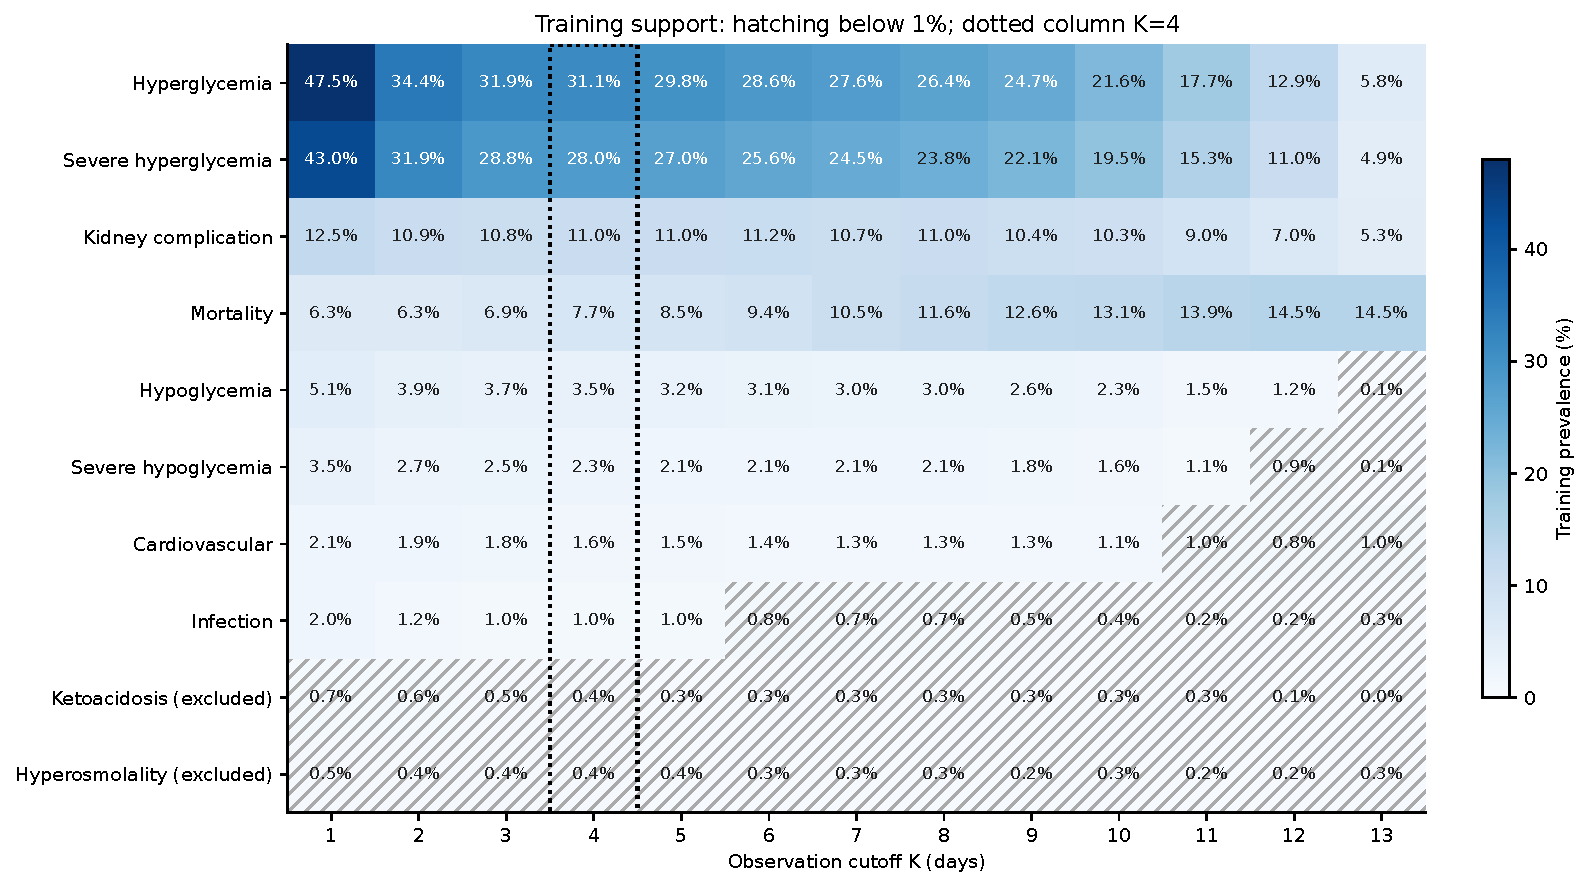
\includegraphics[width=\textwidth]{updated_support_heatmap}
\caption{Prevalence of the ten candidate complications in the original training set. Color indicates the proportion of admissions with an event after cutoff $K$ and through day 14, $(K,14]$. Hatching marks prevalence below 1\%. The dotted outline identifies the cutoff used for outcome selection ($K=4$), and \emph{no head} identifies the excluded outcomes.}
\label{fig:support}
\end{figure}

\subsection{Overall predictive performance and baseline comparisons}
At day four, both comparisons favored clinical intervals (Table~\ref{tab:ladder}). Weighted AUPRC was 0.527 for KB, 0.475 for ss-STraTS, and 0.467 for the SAX interval encoder. The paired gains for KB were 0.053 over ss-STraTS (95\% CI 0.036--0.070) and 0.060 over SAX (0.046--0.076), with $q=0.0012$ for both comparisons. Thus KB improved discrimination even against a model with the same interval encoder. Weighted AUROC also favored KB, and the AUPRC advantage persisted when all outcomes received equal weight.

\begin{table}[htbp]
\centering\small
\caption{Predictive discrimination and length-of-stay error at the four-day observation cutoff.}
\label{tab:ladder}
\resizebox{\textwidth}{!}{\begin{tabular}{lrrrrr}
\toprule
Model & Parameters & Weighted AUPRC & Weighted AUROC & Macro AUPRC & LoS MAE (h) \\
\midrule
Logistic Regression & 25,687 & 0.453 [0.434, 0.475] & 0.751 [0.740, 0.763] & 0.369 & 47.56 \\
Logistic Regression + QA & 26,129 & 0.450 [0.432, 0.472] & 0.751 [0.740, 0.762] & 0.366 & 47.53 \\
\midrule
ss-STraTS & 91,441 & 0.475 [0.456, 0.495] & 0.770 [0.760, 0.781] & 0.370 & 46.27 \\
ss-STraTS + QA & 94,769 & 0.473 [0.456, 0.494] & 0.770 [0.760, 0.781] & 0.360 & 47.48 \\
\midrule
INTERVenE SAX & -- & 0.467 [0.450, 0.488] & 0.762 [0.751, 0.773] & 0.329 & 48.37 \\
INTERVenE KB & $\approx$1.85M & 0.527 [0.510, 0.548] & \textbf{0.803 [0.794, 0.812]} & \textbf{0.402} & \textbf{45.76} \\
INTERVenE KB + QA & $\approx$1.86M & \textbf{0.535 [0.518, 0.555]} & 0.801 [0.791, 0.811] & \textbf{0.402} & 45.85 \\
\bottomrule
\end{tabular}
}
\par\smallskip\parbox{\textwidth}{\footnotesize Parameter counts include prediction heads. QA counts are calculated from the input dimensions. KB totals are approximate. The SAX count was unavailable (Supplementary Methods A). All models were evaluated on the same test admissions. Intervals are 95\% bootstrap intervals clustered by person, with 2,000 valid draws for each primary discrimination summary. Weighted metrics use the number of positive admissions per outcome. Macro AUPRC gives outcomes equal weight. Bold marks the highest discrimination or lowest length-of-stay MAE (LoS, in hours), including ties at the precision shown. Bold values are ranked point estimates.}
\end{table}

Hyperglycemic outcomes accounted for much of the weighted gain, and KB also discriminated well for mortality (Table~\ref{tab:outcomes}). For kidney and cardiovascular complications, the raw-data models were competitive with KB. Only 33 test admissions had an infection, 66 a cardiovascular complication, and 108 severe hypoglycemia, making small differences between models difficult to interpret for these outcomes.

\begin{table}[htbp]
\centering\scriptsize
\caption{Per-outcome discrimination and complication-onset error.}
\label{tab:outcomes}
\resizebox{\textwidth}{!}{\begin{tabular}{lrrrrrrrrr}
\toprule
 & & & \multicolumn{2}{c}{Logistic Regression} & \multicolumn{2}{c}{ss-STraTS} & \multicolumn{3}{c}{INTERVenE} \\
\cmidrule(lr){4-5}\cmidrule(lr){6-7}\cmidrule(lr){8-10}
Outcome & $n_+$ & \% & LR & LR+QA & ST & ST+QA & SAX & KB & KB+QA \\
\midrule
\multicolumn{10}{l}{\textit{AUPRC (higher is better)}} \\
Hyperglycemia & 1427 & 31.65 & 0.450 & 0.449 & 0.489 & 0.496 & 0.494 & 0.578 & \textbf{0.597} \\
Severe hyperglycemia & 1285 & 28.50 & 0.441 & 0.438 & 0.476 & 0.467 & 0.463 & 0.515 & \textbf{0.517} \\
Kidney complication & 545 & 12.09 & 0.589 & 0.587 & 0.582 & 0.578 & 0.556 & 0.585 & \textbf{0.602} \\
Mortality & 329 & 7.30 & 0.584 & 0.578 & 0.552 & 0.570 & 0.609 & \textbf{0.640} & 0.604 \\
Hypoglycemia & 178 & 3.95 & 0.137 & 0.133 & 0.142 & 0.132 & 0.136 & 0.152 & \textbf{0.165} \\
Severe hypoglycemia & 108 & 2.40 & 0.106 & 0.105 & 0.109 & 0.104 & 0.100 & 0.121 & \textbf{0.134} \\
Cardiovascular & 66 & 1.46 & 0.573 & 0.567 & \textbf{0.587} & 0.491 & 0.240 & 0.569 & 0.499 \\
Infection & 33 & 0.73 & 0.073 & 0.069 & 0.027 & 0.041 & 0.034 & 0.062 & \textbf{0.100} \\
\midrule
\multicolumn{10}{l}{\textit{Complication-onset MAE in hours (lower is better)}} \\
Hyperglycemia & 1427 &  & 28.48 & 28.55 & 28.92 & 27.95 & 27.68 & \textbf{25.47} & 25.72 \\
Severe hyperglycemia & 1285 &  & 28.33 & 28.39 & 29.16 & 28.10 & 28.39 & \textbf{27.16} & 27.41 \\
Kidney complication & 545 &  & 32.76 & 32.80 & 34.30 & 33.89 & 33.09 & 32.88 & \textbf{32.11} \\
Mortality & 329 &  & 58.65 & 58.68 & 57.87 & 58.48 & \textbf{56.27} & 56.30 & 57.41 \\
Hypoglycemia & 178 &  & 41.87 & 42.29 & 38.96 & 41.56 & 37.07 & 36.76 & \textbf{36.13} \\
Severe hypoglycemia & 108 &  & 45.09 & 46.80 & 46.62 & 48.22 & 40.66 & 40.47 & \textbf{40.37} \\
Cardiovascular & 66 &  & 40.37 & 39.94 & \textbf{34.95} & 42.42 & 38.76 & 36.40 & 35.89 \\
Infection & 33 &  & 45.57 & 52.78 & 31.62 & 37.24 & 31.11 & 32.30 & \textbf{29.49} \\
\bottomrule
\end{tabular}
}
\par\smallskip\parbox{\textwidth}{\footnotesize LR denotes logistic regression and ST denotes ss-STraTS. Prevalence is expressed as a percentage. The upper block gives AUPRC. The lower block gives onset MAE in hours among admissions with the outcome ($n_+$). Bold marks the highest AUPRC or lowest MAE for each outcome at the precision shown. For mortality, onset MAE measures error in the time to the death-coded end of the visit, including when death occurred after discharge. These rankings compare point estimates. Model families are grouped as in Table~\ref{tab:ladder}.}
\end{table}
\subsection{Length of stay and complication timing}
\noindent\textit{Draft note: Training-median baselines for length of stay and time to each complication remain to be evaluated. The model-to-model timing comparisons below are available; performance relative to these simple constant predictors is pending.}

KB had the lowest mean absolute error for length of stay, at 45.76 hours (95\% CI 44.68--46.80). The corresponding errors were 46.27 hours (45.18--47.36) for ss-STraTS, 47.56 for logistic regression, and 48.37 for SAX (Table~\ref{tab:ladder}). The difference between KB and ss-STraTS was small. Their intervals overlapped, and these separate estimates do not provide a paired test of the difference. With QA, the KB error was similar at 45.85 hours.
The clearest timing differences concerned the glycemic outcomes (Table~\ref{tab:outcomes}, lower block). For hyperglycemia and severe hyperglycemia, onset MAE was 25.47 and 27.16 hours with KB, compared with 28.92 and 29.16 for ss-STraTS. KB+QA had the lowest point estimates for hypoglycemia and severe hypoglycemia (36.13 and 40.37 hours). For the other outcomes, the model with the smallest error varied.

\subsection{Incremental predictive value of guideline assessment}
\label{sec:results-qa}
KB+QA had the highest weighted AUPRC (0.535), but its paired advantage over KB was small and uncertain (0.007, 95\% CI $-0.003$ to 0.018, $q=0.1942$). Macro AUPRC was essentially the same with and without QA. The overall differences on adding QA to logistic regression or ss-STraTS were also inconclusive.

Adding QA to KB changed the AUPRC point estimate by +0.020 for hyperglycemia, +0.014 for hypoglycemia, +0.014 for severe hypoglycemia, and +0.017 for kidney complications. Of these increases, only the one for hyperglycemia remained significant after correction for multiple comparisons (95\% CI 0.005--0.035, $q=0.0380$). Mortality discrimination fell by 0.036 (95\% CI $-0.056$ to $-0.015$, $q=0.0240$), and severe hyperglycemia changed little. Supplementary Tables~S1 and~S2 give the outcome-specific and overall paired comparisons, respectively.

The favorable glycemic estimates concern the outcomes targeted by the recommendations. The earlier clinical study examined how adherence related to those outcomes \citep{oded2027kineret-jbi}. Here the comparison measured how much information an assessment added once the model had seen the physiological history. An association with an outcome can therefore coexist with little gain in prediction, and these predictive differences cannot establish whether adherence prevents complications.

\subsection{Recording conditions relative to the prior ICU study}
In the first 96 hours, heart rate and temperature were recorded more frequently in the raw MIMIC-IV data used for INTERVenE than in Kineret \citep{oded2026intervene}. Median daily counts were 12.5 versus 2 for heart rate and 3.5 versus 1.75 for temperature. Glucose showed the reverse pattern, with 4 readings per day in Kineret versus 2.75 in MIMIC-IV, consistent with Kineret's focus on inpatient hyperglycemia. INTERVenE-Enc outperformed raw-observation models in both studies when fitted to each cohort separately. The comparison documents the different recording conditions under which the architecture performed well. It cannot attribute differences in performance to recording frequency. Supplementary Tables~S4--S6 give measurement frequencies and gaps between readings.

\subsection{Performance across observation cutoffs}
KB outperformed ss-STraTS and SAX at every daily cutoff from day two to day six. At each cutoff, the paired intervals for the difference in weighted AUPRC excluded zero (Figure~\ref{fig:windows}). Later cutoffs select longer admissions and leave less time for an outcome to occur, so changes across cutoffs cannot establish the benefit of an extra day of observation.

For KB, the overall gain from QA remained uncertain at every cutoff. For ss-STraTS, QA improved discrimination at day two ($\Delta$ AUPRC 0.013, 95\% CI 0.002--0.022, $q=0.0150$), indicating that an early guideline assessment can also help a model of individual observations. We adjusted for multiple comparisons separately at each cutoff.
\begin{figure}[htbp]
\centering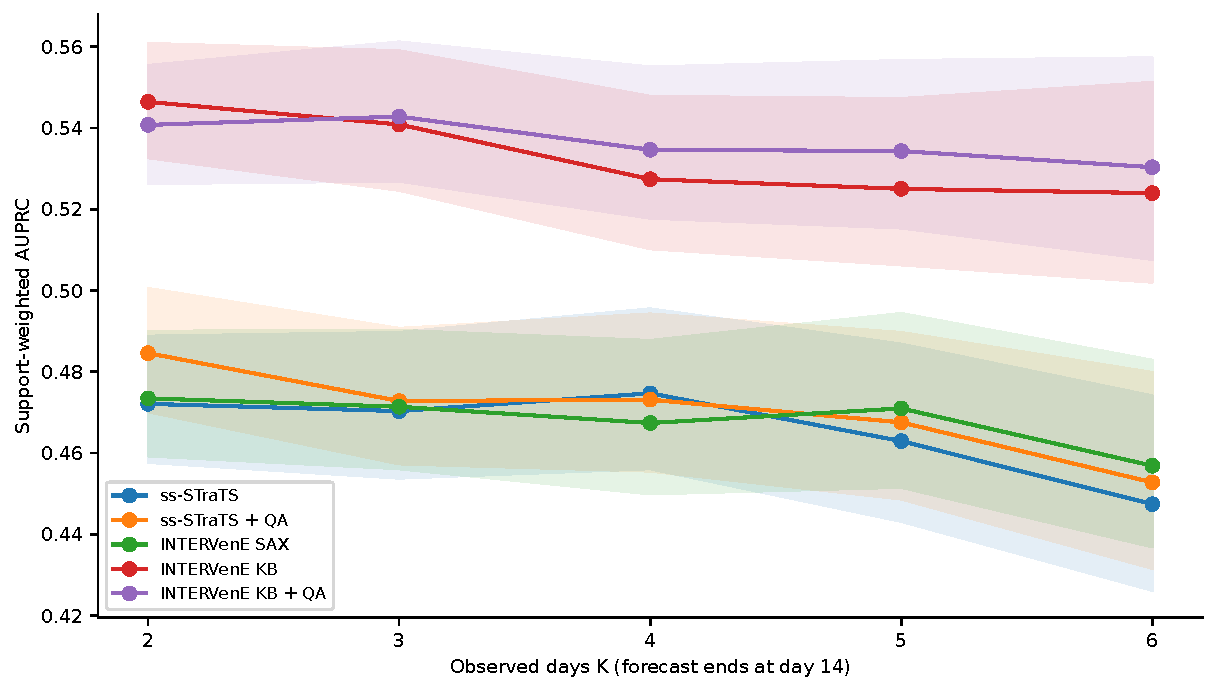
\includegraphics[width=.9\textwidth]{updated_window_sensitivity}
\caption{Weighted AUPRC for predictions made from day two to day six, with follow-up through day 14. Model weights were fixed across cutoffs. Shading indicates 95\% intervals.}
\label{fig:windows}
\end{figure}

\subsection{Transfer to held-out hospitals}
KB retained discrimination at all six hospitals when each was held out from training (Table~\ref{tab:loo}). Weighted AUPRC ranged from 0.431 to 0.539 across hospitals and weighted AUROC from 0.725 to 0.828. The corresponding pooled estimates, 0.527 and 0.803, lay within these ranges, although some hospitals had lower scores. Each hospital contributed a different patient population, so these comparisons cannot quantify the loss attributable to moving a model to a new site.

\begin{table}[htbp]
\centering\small
\caption{KB performance when the evaluated hospital is excluded from fitting.}
\label{tab:loo}
\resizebox{\textwidth}{!}{\begin{tabular}{lrrrr}
\toprule
Held-out hospital & Admissions & PR reference & AUPRC (95\% CI) & AUROC (95\% CI) \\
\midrule
Barzilai University Medical Center & 5,978 & 0.236 & 0.516 [0.500, 0.534] & 0.788 [0.779, 0.797] \\
Bnai Zion Medical Center & 3,253 & 0.266 & 0.539 [0.520, 0.563] & 0.776 [0.765, 0.788] \\
Galilee Medical Center & 5,899 & 0.158 & 0.481 [0.462, 0.501] & 0.829 [0.820, 0.837] \\
Hillel Yaffe Medical Center & 5,063 & 0.228 & 0.464 [0.449, 0.481] & 0.771 [0.762, 0.780] \\
Tzafon Medical Center (Poria) & 2,388 & 0.251 & 0.431 [0.409, 0.457] & 0.725 [0.710, 0.740] \\
Shamir Medical Center & 7,348 & 0.264 & 0.514 [0.499, 0.530] & 0.770 [0.762, 0.779] \\
\bottomrule
\end{tabular}
}
\par\smallskip\parbox{\textwidth}{\footnotesize The precision--recall reference is the mean outcome prevalence at each hospital, weighted by positive counts ($\sum_j p_j^2/\sum_j p_j$). Supplementary Table~S3 gives the individual prevalences. At Bnai Zion, only 1,710 of 2,000 bootstrap draws were valid, below the prespecified threshold for reliable intervals. All other aggregate intervals had 2,000 valid draws.}
\end{table}
\noindent\textit{Author note: Confirm with coauthors whether hospitals may be identified by name; anonymize consistently if required.}

At every held-out hospital, AUPRC exceeded the reference calculated from that hospital's outcome prevalences. The six KB fits alone took more than a week, which made repeating the analysis for all baseline models impractical. The comparison with other models therefore comes from the pooled test set. Supplementary Table~S7 breaks down pooled-model performance by age, sex, and hospital. Infection occurred in only two test admissions among patients younger than 55 and in none of the 495 test admissions at Bnai Zion, where aggregate discrimination across all eight outcomes was consequently undefined. Supplementary Table~S8 reports calibration.

\subsection{Embedding structure}
At a fixed timestamp, the closest embeddings were the START and END of the same concept (median cosine distance 0.180). Distances increased from pairs sharing an abstraction (0.226) to those sharing only an underlying variable (0.443) and those with different underlying variables (0.590). Figure~\ref{fig:embedding} shows this organization for the whole vocabulary and in more detail for glucose. The trained embeddings preserved the relationship between a concept's boundaries and its place in the clinical hierarchy. Whether an END token attends to the START of its own interval is a separate question that embedding distances cannot answer.
\begin{figure}[p]
\centering
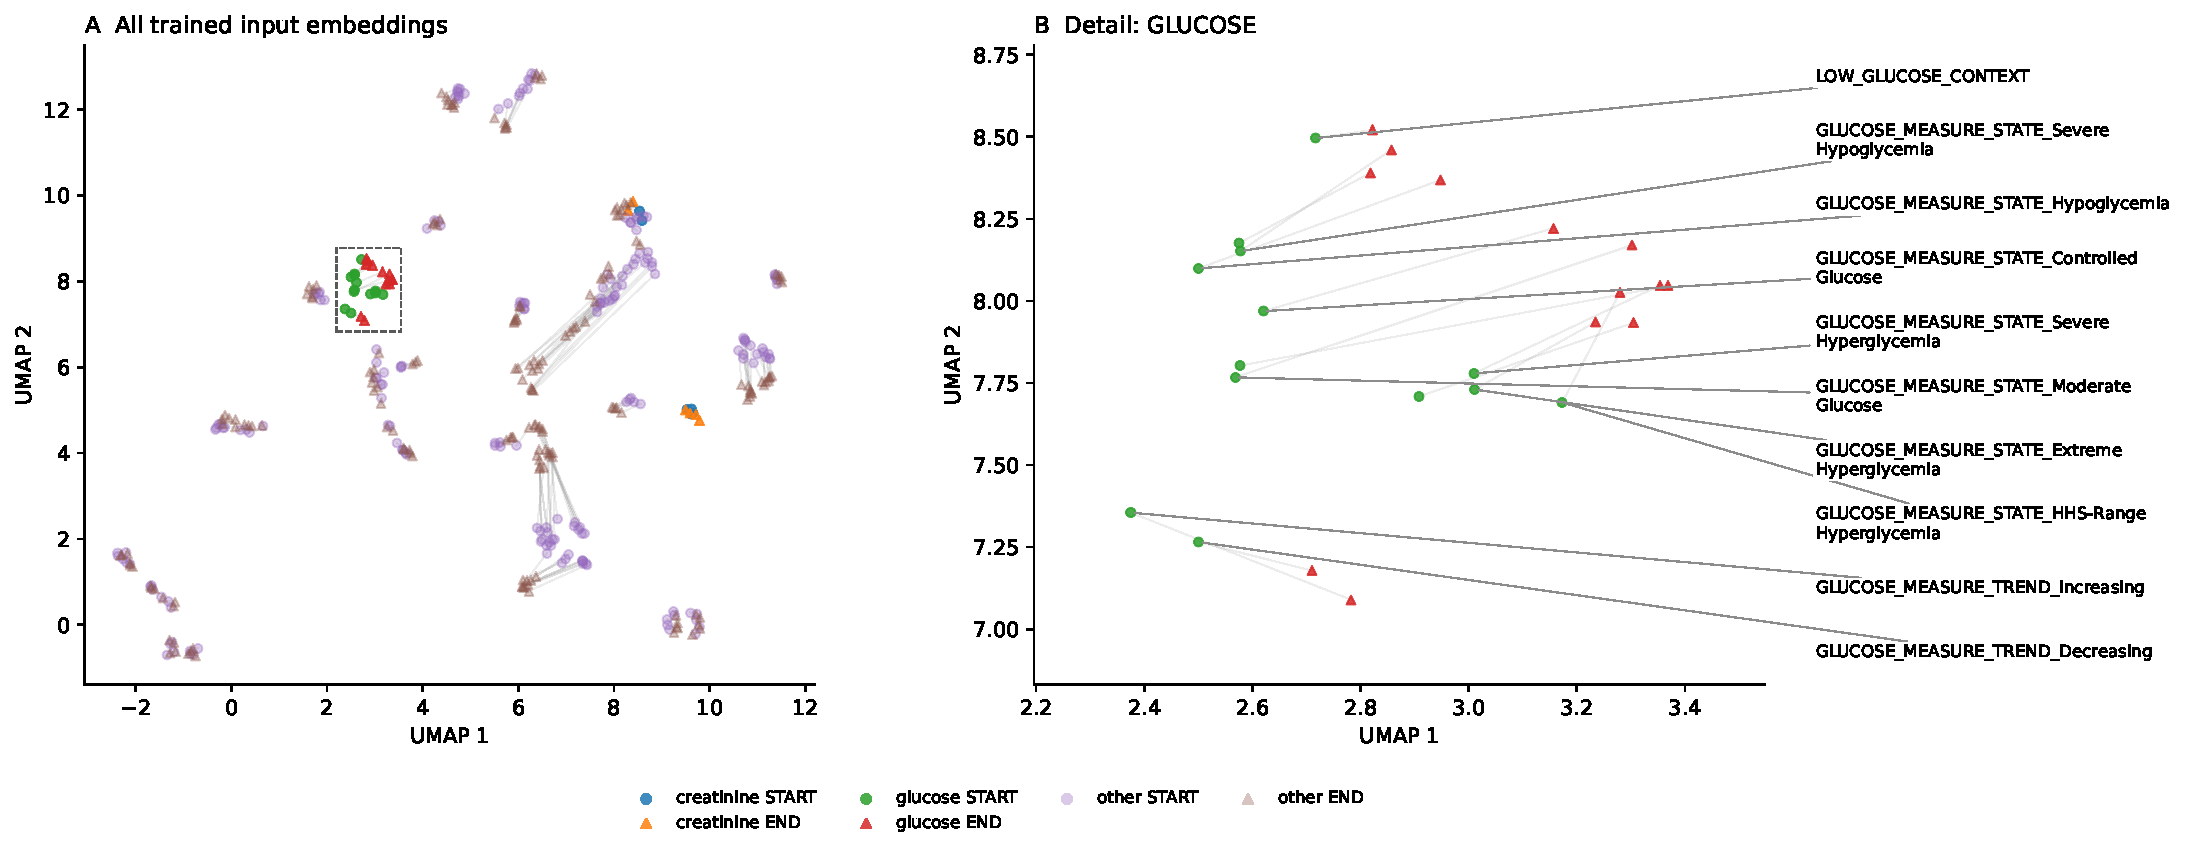
\includegraphics[width=.65\textwidth,trim=0 45 610 0,clip]{updated_embedding_umap}\\[8pt]
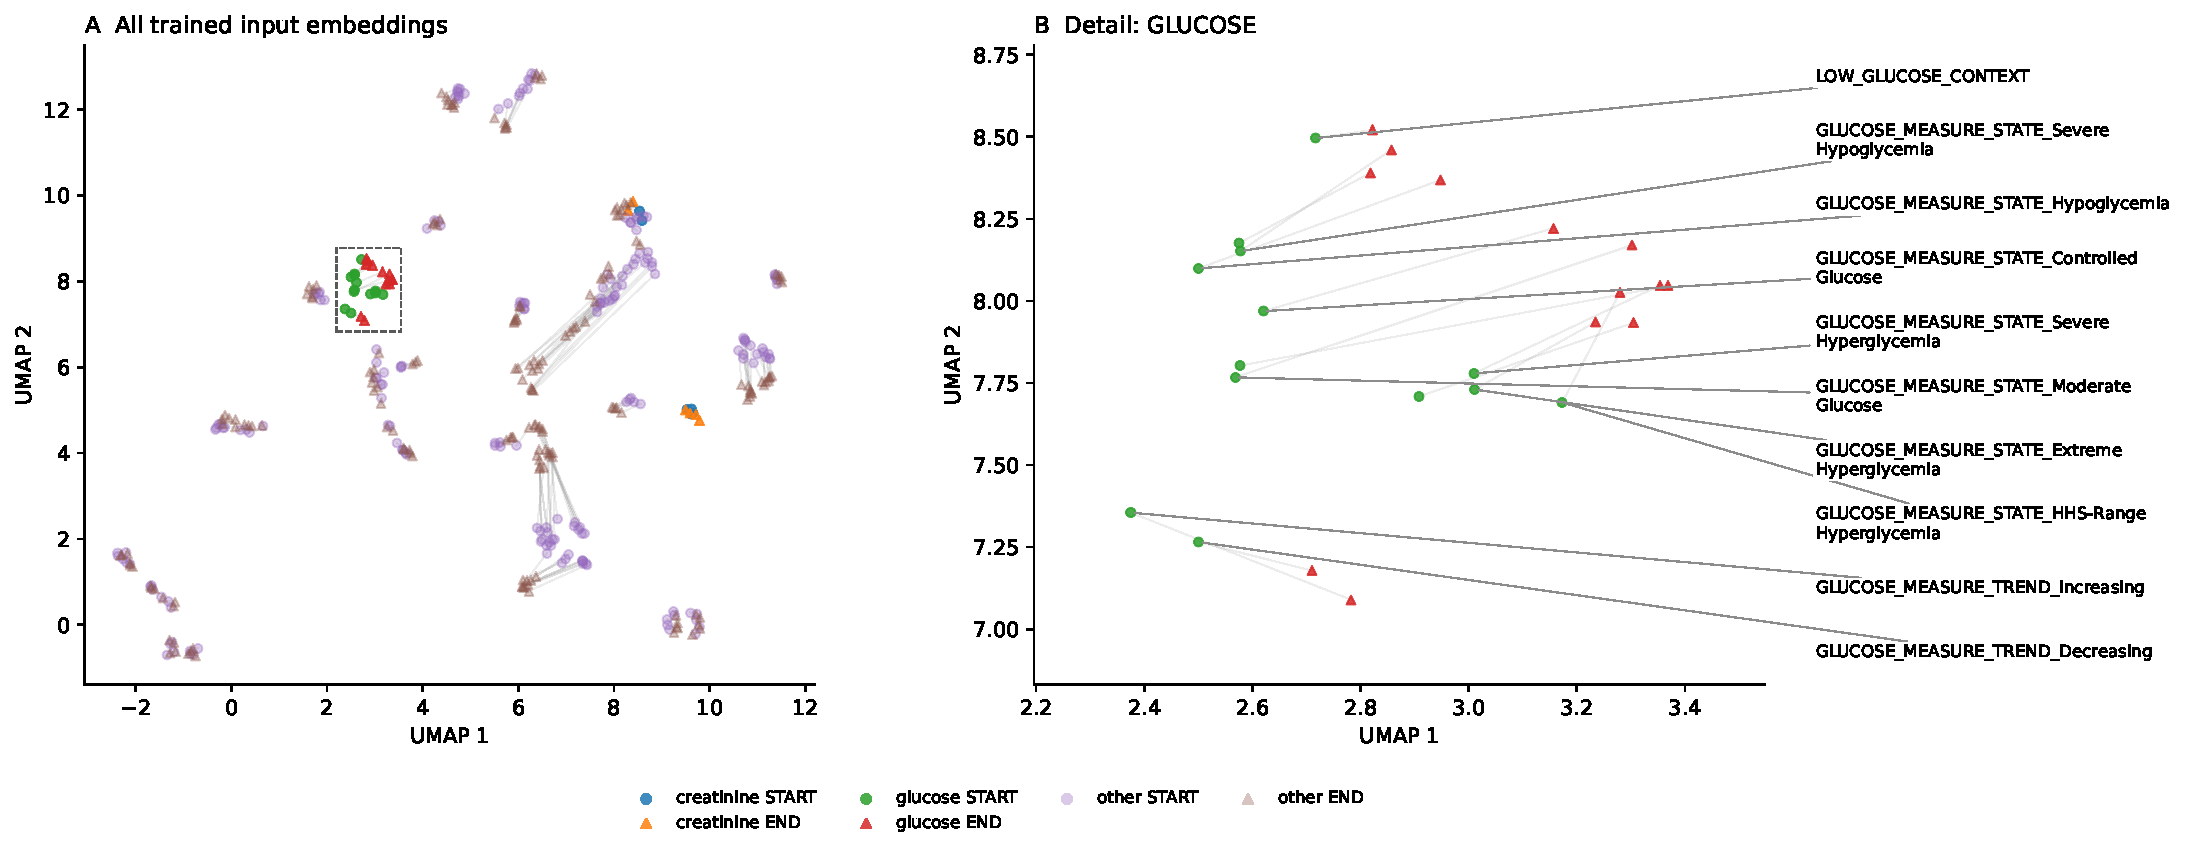
\includegraphics[width=\textwidth,trim=480 45 0 0,clip]{updated_embedding_umap}
\caption{Trained input embeddings at a fixed timestamp. The upper panel shows the UMAP projection of the vocabulary. The lower panel enlarges the glucose family in the same projection. Circles denote START tokens and triangles denote END tokens. The encoder incorporates the clinical hierarchy, and the reported cosine distances were calculated in the original embedding space.}
\label{fig:embedding}
\end{figure}

\subsection{Named-concept attribution and the previous clinical findings}
In KB+QA, the clinical token at a given position identifies a state, trend, event, context, or guideline assessment. Summing transcoder contributions at positions with the same name lets us report a contribution from \emph{decreasing glucose}, for example, even when that trend spans several readings. The vocabulary supplies the name, and the transcoder estimates the model's sensitivity at each occurrence. Clinical states accounted for many of the largest contributions. Every outcome had a QA pattern among its top 30 concepts, although the highest-ranked QA pattern ranged from seventh to twenty-fourth across outcomes.

A falling glucose trend contributed toward higher predicted hypoglycemia risk. When the insulin-after-hyperglycemia pattern was scored false, it contributed toward lower predicted risk and ranked seventh for both hypoglycemia outcomes. In the clinical study, greater adherence to this recommendation was associated, after propensity weighting, with higher odds of hypoglycemia (OR 1.283, 95\% CI 1.163--1.416) and lower odds of severe hyperglycemia (OR 0.220, 0.202--0.239) \citep{oded2027kineret-jbi}. The direction of the attribution is consistent with this trade-off. A pattern scored false leaves open how much insulin the patient received and why care differed from the recommendation.

Routine glucose monitoring was the highest-ranked QA concept for mortality and contributed toward lower predicted risk. The clinical study also found lower odds of 30-day mortality with greater adherence to routine monitoring after propensity weighting (OR 0.870, 95\% CI 0.809--0.937) \citep{oded2027kineret-jbi}. That analysis accounted for measured confounders, although residual confounding was possible. The attribution describes a predictive association and cannot establish that monitoring prevented deaths. Despite the direction of this particular contribution, adding all QA inputs reduced the model's ability to distinguish admissions ending in a death marker from those without one during the forecast period.

For all 300 admissions, attaching the transcoders left the original risk predictions unchanged (maximum absolute difference in risk logits, 0). Reconstruction was less complete. Across the four layers, the transcoders explained only part of the variance in held-out layer outputs ($R^2=0.396$--$0.514$). The encoder continued to use its original layer outputs for prediction. The unexplained variance therefore limits the feature-based explanation, even though the predictions themselves were unchanged. Agreement with selected findings from the clinical study lends these exploratory explanations clinical plausibility. Supplementary Table~S9 gives reconstruction and sparsity by layer. Table~S10 lists the highest-ranked QA concepts.

\subsection{Stability of the clinical abstractions}
For the 500 people in the perturbation analysis, the Mediator assigned the same state label to 97.6\% of covered time and the same trend label to 98.0\% after we added noise of 5\% of local threshold spacing. When we removed 10\% of observations, agreement was 97.4\% for states and 95.3\% for trends. The corresponding losses of baseline coverage were 2.0\% and 3.2\%. These estimates describe the stability of numeric states and trends under modest changes in the measurements. QA patterns and downstream predictions were outside this analysis. Supplementary Table~S11 reports intervals and coverage for each perturbation.

\section{Discussion}
\label{sec:discussion}
\subsection{Prediction across care settings}
In six Israeli general hospitals, INTERVenE-Enc distinguished patients who subsequently developed complications more accurately than ss-STraTS. At day four, the difference in weighted AUPRC was 0.053 (95\% CI 0.036--0.070), and the advantage persisted at each daily cutoff from day two to day six. The models differed in size, so this comparison establishes their relative performance in the configurations studied. The advantage over ss-STraTS extends the earlier finding in MIMIC-IV intensive care records to general inpatient care in another health system \citep{oded2026intervene}. Differences in timing accuracy were more modest. They were clearest for the onset of hyperglycemia, while the most accurate model varied across other complications.

The two settings offered different views of a patient's course. During the first four days, the median number of heart-rate readings per day was two in Kineret and 12.5 in MIMIC-IV. For glucose, it was four in Kineret and 2.75 in MIMIC-IV. A Kineret record could therefore document glycemic changes relatively frequently while leaving hours between observations of vital signs. The encoder performed well under both recording patterns when fitted to local data. Case mix and outcome definitions also differed between the studies, limiting what can be attributed to recording frequency alone.

Within Kineret, a model fitted at five hospitals retained discrimination at the sixth. KB exceeded the local prevalence reference at every site, although weighted AUPRC ranged from 0.431 to 0.539. Differences in case mix, event frequency, and local recording practices matter when interpreting that range. At one hospital, rare events made the aggregate interval unreliable. Because the hospital holdouts included only KB, the evidence for its advantage over other models comes from the pooled comparison.

\subsection{What the clinical knowledge base contributed}
In the ICU study, statistically defined intervals preserved much of the encoder's performance, while the clinical vocabulary made it possible to identify which states and trends contributed to a prediction \citep{oded2026intervene}. In Kineret, the choice of intervals also mattered for discrimination. Clinical intervals improved weighted AUPRC by 0.060 (95\% CI 0.046--0.076) over SAX in the same encoder architecture. Much of the gain came from glycemic outcomes, for which the knowledge base contains detailed definitions, and the advantage persisted when each outcome received equal weight.

SAX indicates which statistical band a variable occupied over a given period. A clinical interval can express that glucose remained elevated, that it was falling, or that a sequence of observations met the criteria for a clinical event. The knowledge base was developed for inpatient diabetes care and mapped to the Kineret hospitals' measurement and treatment codes \citep{oded2027kineret-jbi}. This close fit to the clinical question may help explain its advantage. Thresholds, timing rules, vocabulary, and access to derived events all changed together, however. The experiment measures their combined value and leaves open how much each contributed or how well the same approach would work in another specialty.

\subsection{What guideline assessment added}
The clinical study associated adherence to particular recommendations with subsequent outcomes \citep{oded2027kineret-jbi}. In the present study, each guideline score summarized measurements and treatments already represented in the clinical history. Making those relationships explicit improved discrimination for subsequent hyperglycemia and reduced it for mortality. The overall difference was small and uncertain, and macro AUPRC was essentially the same with and without QA. A recommendation can therefore be clinically relevant even when an assessment of adherence adds little to what the model can infer from the record.

The hypoglycemia findings illustrate what the clinical vocabulary makes visible. A raw-observation model can assign a contribution to a glucose reading at a particular time. The interval model can assign one to a fall in glucose or to the timing of insulin after an elevated reading. A falling glucose trend contributed toward higher predicted hypoglycemia risk, and an insulin-after-hyperglycemia pattern scored false contributed toward lower risk. These directions are consistent with the clinical study, in which greater adherence to that recommendation was associated with fewer episodes of severe hyperglycemia and more episodes of hypoglycemia \citep{oded2027kineret-jbi}. They also fit the clinical rationale for coordinating glucose monitoring, insulin, and nutrition in hospital \citep{ada2026hospital}. The pattern score alone cannot resolve the dose, actual intake, or reason for a treatment decision.

For mortality, the direction of an individual contribution and the overall change in discrimination are especially informative together. Routine glucose monitoring contributed toward lower predicted risk, consistent with the association with 30-day mortality in the clinical study. Yet the model with all QA inputs was less accurate at identifying admissions with a death-coded terminal marker in the forecast window. An attribution describes how the fitted model used a pattern. It cannot tell us what would happen if clinicians monitored glucose more often.

\subsection{Interpreting a contribution to predicted risk}
A name such as \emph{decreasing glucose} comes from the clinical rule that defined the interval. The embedding analysis showed that the encoder retained relationships within that vocabulary, with the two boundaries of the same concept closer together than concepts from different clinical families. In a separate test, modest noise or removal of measurements left most covered time with the same numeric state or trend label. The stability of QA patterns and downstream risk estimates remains untested.

Identifying a clinically recognizable input is only part of explaining a prediction. The transcoder estimates sensitivity at occurrences of that input through a sparse approximation to each layer's output. Its reconstruction explained part of the variance on held-out data ($R^2=0.396$--$0.514$). Attaching the transcoders preserved the original predictions across 300 admissions, but the unexplained variation limits how fully the attributions can account for an individual prediction.

\subsection{Limitations and clinical implications}
\label{sec:discussion-limits}
The day-four results apply to adults with diabetes or early hyperglycemia whose records extended beyond four days. Shorter admissions were outside that evaluation. A recorded onset also depends on when clinicians measured the patient or documented an event. We applied the date restriction to an evaluation of previously fitted models, and the intervals quantify sampling variation across patients for those models. Rare events limit the precision of some hospital and subgroup estimates.

Mortality timing has a further limitation. For a death recorded after discharge, the model predicts the time of the death-coded visit end, so its onset error cannot be interpreted as error in predicting the actual time of death.

Guideline scores reflect what can be reconstructed from the record. For example, meal-related rules used assumed meal times, and the summaries assigned each assessment to its recorded start. Before using these scores during care, it would be necessary to establish when all the observations needed to calculate them would have been available. Illness severity and the circumstances prompting treatment can also influence both recorded adherence and subsequent risk. The agreement between selected attributions and the clinical study must be read in that context. Both analyses draw on the same records.

For a clinician deciding whether to observe a patient more closely, the timing of a complication matters alongside its likelihood. Comparisons with training-median predictions are still needed to interpret the absolute errors for both onset and length of stay. For predicted probabilities, the clinical interval model showed closer agreement with observed outcomes than ss-STraTS in the pooled test set (mean expected calibration error 0.0122 and 0.1268, respectively). Choosing a threshold for action would require checking calibration at the intended hospital and weighing missed events against false alerts.

\section{Conclusion}
\label{sec:conclusion}
In adults hospitalized with diabetes or hyperglycemia, clinically defined intervals gave INTERVenE-Enc better discrimination than statistically defined intervals, and the clinical encoder outperformed models of individual observations. Together with the ICU findings, this supports the approach in two health systems with different recording practices and with models fitted in each setting. In Kineret, guideline assessments improved discrimination for hyperglycemia, reduced it for mortality, and offered no clear overall gain. For every outcome, however, the model's sensitivity could be traced to named patterns of care as well as to the patient's physiological history.


\section*{CRediT Authorship Contribution Statement}
\textbf{Shahar Oded:} Conceptualization, Methodology, Software, Validation,
Formal analysis, Data curation, Visualization, Writing---original draft.
\textbf{Yuval Shahar:} Conceptualization, Methodology, Supervision, Funding
acquisition, Writing---review \& editing.
\textbf{Erez Shalom:} Resources, Project administration, Writing---review \&
editing.
\textbf{Amir Bashkin:} Investigation, Resources, Writing---review \& editing.
\textbf{Leonard Saiegh:} Investigation, Resources, Writing---review \& editing.
\textbf{Dror Cantrell:} Investigation, Resources, Writing---review \& editing.
\textbf{Irit Wirsansky:} Investigation, Resources, Writing---review \& editing.
\textbf{Muhamad Badarne:} Investigation, Resources, Writing---review \& editing.
\textbf{Irena Barash:} Investigation, Resources, Writing---review \& editing.
\textbf{Avivit Cahn:} Conceptualization, Investigation, Writing---review \&
editing.
\textbf{Irit Hochberg:} Conceptualization, Methodology, Validation,
Resources, Supervision, Writing---review \& editing.

\section*{Funding}
This research was funded by the Israeli Ministry of Science and Technology
Kineret Grant No.~0006850 (Governmental Project No.~1001701806), the Israeli
National Health Policy Grant No.~2020/284, the Israel Precision Medicine
Partnership (IPMP) Grant No.~3543/21, and the European Union's Horizon Europe
research and innovation programme under Grant Agreement No.~101156210
[CARAMEL]. The funders had no role in study design, data collection and
analysis, decision to publish, or preparation of the manuscript.

\section*{Declaration of Competing Interest}
Several of the authors contributed to the national position paper whose
implementation informs the QA arm of this study. The authors declare no
competing financial interests or personal relationships that could have
appeared to influence the work reported in this paper.

\section*{Data and Code Availability}
The study software covers temporal abstraction, cohort construction, and model evaluation.
% Verify repository release visibility before submission.

\begin{itemize}\setlength{\itemsep}{.1em}
\item Temporal Mediator and its knowledge base for abstraction and guideline assessment. \url{https://github.com/shaharoded/Mediator}
\item Kineret extraction and cohort construction. \url{https://github.com/shaharoded/Kineret-ETL}
\item INTERVenE-Enc reference implementation. \url{https://github.com/shaharoded/INTERVenE-Enc}
\item STraTS reference implementation for the supervised comparator.\newline{\small\url{https://github.com/shaharoded/Medical-Transformers-Benchmark}}
\item Kineret prediction code, training configurations, and aggregate results. \url{https://github.com/shaharoded/Kineret-Prediction}
\end{itemize}

Patient-level records were processed within the hospital computing environment. The study approvals restrict access to those records. The reported tables and figures are based on aggregate outputs.

\section*{Ethics Approval}
The institutional Helsinki committee at each participating center approved the study under a common protocol (NHR-0152-23). Local approvals were granted by Galilee Medical
Center (NHR-0152-23), Hillel Yaffe Medical Center (HYMC-0074-24), Shamir
Medical Center (ASF-0117-24), Tzafon Medical Center (POR-0047-24), Barzilai
University Medical Center (BRZ-0059-24), and Bnai Zion Medical Center
(BNZ-0067-24). The committees waived informed consent for this retrospective analysis of de-identified records without patient contact.

\section*{Acknowledgements}
The authors thank the Kineret project team for building and maintaining the multicenter data warehouse and the Helsinki committee coordinators at the participating centers for their assistance.

\bibliographystyle{elsarticle-num}
\bibliography{references}

\end{document}
